% -*- root: ../supcom.tex -*-

\section{Matrix-vector multiplication} % (fold)
\label{sec:matrix_multiplication}

This section is based on the notes found at \url{http://www.hpcc.unn.ru/mskurs/ENG/DOC/pp07.pdf}.

\subsection{Problem statement} % (fold)
\label{sub:problem_statement}
The result of multiplying the matrix $A$ of order $m\times n$ by vector $b$, consisting of $n$ elements, is the vector $c$ of size $m$, each $i$-th element of which is the result of the inner multiplication of the $i$-th matrix $A$ row $a_i$ by vector $b$:
\begin{equation}
  c_i = \sum_{j=0}^{n-1} a_{ij}b_j, \quad 0\leq i \leq m-1
\end{equation}

Each operation includes multiplying the matrix row elements by the elements of vector $b$ ($n$ operations) and the following summing the obtained products ($n-l$ operations). The total number of necessary scalar operations is the value
\begin{equation}
  T_1 = m \cdot (2n-1)
\end{equation}
% subsection problem_statement (end)

\subsection{Data distribution} % (fold)
\label{sub:data_distribution}
While executing the parallel algorithm of matrix-vector multiplication, it is necessary to distribute not only the matrix $A$, but also the vector $b$ and the result vector $c$. The vector elements can be duplicated, i.e. all the vector elements can be copied to all the processors of the multiprocessor computer system, or distributed among the processors. In case of block partitioning of the vector consisting of $n$ elements, each processor processes the continuous sequence of $k$ vector elements (we assume that the vector size $n$ is divisible by the number of processors $p$, i.e. $n = k·p$).

Let us make clear, why duplicating vectors $b$ and $c$ among the processors is an admissible decision (for simplicity further we will assume that $m=n$). Vectors $b$ and $c$ consist of $n$ elements, i.e. contain as much data as one matrix row or column. If the processor holds a matrix row or column and single elements of the vectors $b$ and $c$, the total size of used memory is the order $O(n)$. If the processor holds a matrix row (column) and all the elements of the vectors $b$ and $c$, the total number of used memory is the same order $O(n)$. Thus, in cases of vector duplicating and vector distributing the requirements to memory size are equivalent.
% subsection data_distribution (end)

\subsection{Matrix-vector multiplication in case of rowwise data decomposition} % (fold)
\label{sub:matrix_vector_multiplication_in_case_of_rowwise_data_decomposition}
To execute the basic subtask of inner multiplication the processor must contain the corresponding row of matrix $A$ and the copy of vector $b$. After computation completion each basic subtask determines one of the elements of the result vector $c$.

To combine the computation results and to obtain the total vector $c$ on each processor of the computer system, it is necessary to execute the all gather operation, in which each processor transmits its computed element of vector $c$ to all the other processors. This can be executed, for instance, with the use of the function MPI\_Allgather of MPI library.

The general scheme of informational interactions among subtasks in the course of computationS is shown in Figure~\ref{fig:rowwise-scheme}.

\begin{figure}[htbp]
  \centering
  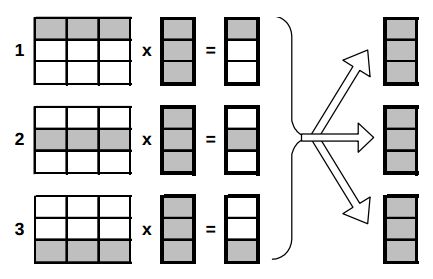
\includegraphics[width=0.5\textwidth]{illustrations/matrix-vector-product/rowwise.png}
  \caption{Computation scheme for parallel matrix-vector multiplication base on rowwise striped matrix partitioning.}
  \label{fig:rowwise-scheme}
\end{figure}


\subsubsection{Efficiency analysis} % (fold)
\label{ssub:efficienct_analysis}
Let us consider the time complexity of the algorithm of matrix-vector multiplication. If matrix $A$ is square $(m=n)$, the sequential algorithm of matix-vector multiplication has the complexity
\begin{equation}
  T_1 = n(n-1+n)\approx 2n^2 = O(n^2)
\end{equation}
In case of parallel computations each processor performs multiplication of only a part (stripe) of the matrix $A$ by the vector $b$. The size of these stripes is equal to $n/p$ rows. In case of computing the inner product of one matrix row by a vector, it is necessary to perform the $n$ multiplications and $(n-l)$ additions. Therefore, computational complexity of the parallel algorithm is determined as:
\begin{equation}
  T_p = \frac{n(n-1+n)}{p} \approx \frac{2n^2}{p} = O(\frac{n^2}{p})
\end{equation}

Taking into accoun this estimation, the criteria of speedup and efficiency of the parallel
\begin{align}
  S_p &= \frac{T_1}{T_p} = \frac{n^2}{n^2/p} = p \\
  E_p &= \frac{T_1}{pT_p} = \frac{n^2}{p(n^2/p)} = 1
\end{align}
These estimations of the computation execution time are expressed in the number of operations. Besides, they are formed \emph{without} taking into consideration the execution of data communication operations. Let us use the above mentioned assumptions that the executed multiplications and additions are of equal duration $\tau_F$.

The computation time of the parallel algorithm is
\begin{equation}
  T_p(calc) = \# rows \times \# ops/row \times \tau_F = \frac{n}{p} \cdot (2n-1) \cdot \tau_F
\end{equation}

After doing the calculations, we use MPI\_Allgather to gather all the $c$-parts on all processors. This works using a binary tree, and so the gather operation can be performed in $\log_2 p$ iterations. In the first iteration, each process sends its part (of size $n/p$) to another process, which in turn will send its own part plus the part it received (total size $2n/p$) on to the next process in the next iteration; thus, the amount of data to be sent doubles in each iteration. As a result, the all gather operation execution time when the hockney model is used can be represented as
\begin{equation}
  T_p (comm) = \sum_{i=1}^{\log_2 p} \left( \tau_S + 2^{i-1} w \frac{n}{p} \gamma \right)
  = \tau_S\log_2 p + w \frac{n}{p} \left( 2^{\log_2 p} -1 \right) \gamma
\end{equation}
where $w$ is the size of each element. Thus, the total time of parallel algorithm execution is
\begin{equation}
  T_p = \frac{n}{p} (2n-1) \tau_F + \tau_S \log_2 p + w \frac{n}{p}(p-1)\gamma
\end{equation}

% subsubsection efficienct_analysis (end)

Note that in this case, we end up with the complete $c$ vector on all processes.

% subsection matrix_vector_multiplication_in_case_of_rowwise_data_decomposition (end)

\subsection{Matrix-vector multiplication in case of columnwise data decomposition} % (fold)
\label{sub:matrix_vector_multiplication_in_case_of_columnwise_data_decomposition}
At the starting point of the parallel algorithm of matrix-vector multiplication each basic task $i$ carries out the multiplication of its matrix $A$ column by element $b_i$. As a result, vector $c'(i)$ (the vector of intermediate results) is obtained in each subtask. The subtasks must further exchange their intermediate data in order to obtain the elements of the result vector $c$ (element $j$, of the partial result $c'(i)$ of the subtask $i$ must be sent to the subtask $j$). This all-to-all communication or total exchange is the most general communication procedure and may be executed with the help of the function MPI\_Alltoall of MPI library. After the completion of data communications each basic subtask $i$ will contain $n$ partial values $c'_i(j)$. Element $c_i$ of the result vector $c$ is determined after the addition of the partial values (see Figure~\ref{fig:colwise}).

\begin{figure}[htbp]
  \centering
  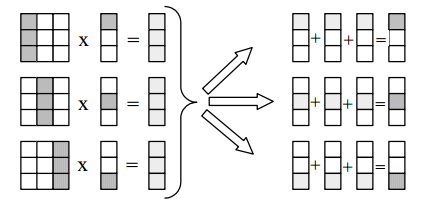
\includegraphics[width=.5\textwidth]{illustrations/matrix-vector-product/column.png}
  \caption{Computation scheme for parallel matrix-vector multiplication based on columnwise striped matrix decomposition. Note that here, we only end up with part of the (summed) $c$ vector on each process.}
  \label{fig:colwise}
\end{figure}



\subsubsection{Efficiency analysis} % (fold)
\label{ssub:efficienct_analysis}
As previously, let matrix $A$ be square, i.e. $m=n$. At the first stage of computations each processor multiplies its matrix columns by the vector $b$ elements. The obtained values are summed for each matrix row separately:
\begin{equation}
  c_s'(i) = \sum_{j=j_0}^{j_{l-1}} a_{sj}b_j, \quad 0\leq s < n
\end{equation}
where $j_0$ and $j_{l-1}$ are the initial and final column indeces of the subtasks $0\leq i <n$. As the sizes of matrix stripes and the block of the vector $b$ are equal $n/p$, the time complexity of such computations may be estimated as
\begin{equation}
  T' = \frac{n(n-1+n)}{p} \approx \frac{n^2}{p}
\end{equation}
operations. After the subtasks have exchanged the data at the second stage of computations each processor sums the obtained values up for its block of the result vector $c$. The number of the summed values for each element $c_i$ of vector $c$ conincides with the number of processors $p$. The size of result vector block is equal to $n/p$. Thus, the number of operations carried out for the second stage appears to be equal to
\begin{equation}
  T'' = \frac{n}{p} p = n
\end{equation}
Thus the total computation time is
\begin{equation}
  T_p = T' + T'' = \frac{n^2}{p} + n \approx \frac{n^2}{p}
\end{equation}
With regards to the relations obtained the speedup and the efficienct of the parallel algorithm may be expressed as follows:
\begin{equation}
  S_p = \frac{T_1}{T_p} = \frac{n^2}{n^2/p} = p, \quad E_p = \frac{T_1}{pT_p} = \frac{n^2}{p(n^2/p)} = 1
\end{equation}

Now let us consider more accurate relations for estimation of the time of parallel algorithm execution. With
regard to the above discussion the execution time of the parallel algorithm computations may be estimated by means
of the following expression:
\begin{equation}
  T_p (calc) = (\frac{n}{p}(\frac{n}{p} - 1 + \frac{n}{p}) \cdot p + \frac{n}{p} \cdot p )\tau_F
   = \left[ n (2 \frac{n}{p} -1  ) + n \right] \cdot \tau_F
\end{equation}

% subsubsection efficienct_analysis (end)



% section matrix_vector_multiplication_in_case_of_columnwise_data_decomposition (end)




% section matrix_multiplication (end)
